
% \usepackage{pstricks}
% \usepackage{pgfplots}
% \usepackage{tikz}
\usetikzlibrary{
	shapes.geometric,
	arrows,
	backgrounds,
	positioning,
	arrows.meta
}

% remove indent
\let\svtikzpicture\tikzpicture
\def\tikzpicture{\noindent\svtikzpicture}

% Defining styles for blocks
\tikzset{
	block/.style 2 args = {
			rectangle,
			font=\small\bfseries\color{#2},
			% draw=white,
			draw=black,
			line width = 0.18mm,
			fill=#1,
			text width=16mm,
			text centered,
			rounded corners = 0.5mm,
			minimum height=10mm
		},
	block/.default = {RoyalBlue}{white}
}

\tikzset{
	sum/.style ={draw,circle,fill=white,minimum size = 1mm}
}

\tikzset{
	dot/.style = {circle, fill, minimum size=#1,
			inner sep=0mm, outer sep=0mm},
	dot/.default = {0.7mm}
}


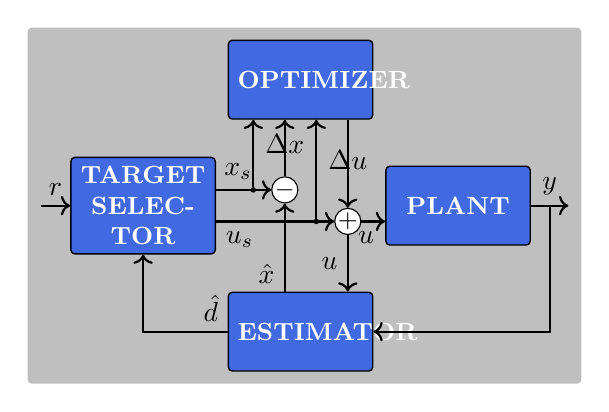
\begin{tikzpicture}[auto,framed, background rectangle/.style={fill=lightgray,rounded corners=0.5mm}]

	% blocks 
	\node [coordinate] (input) at (-33mm,0mm){};
	\node [coordinate] (output) at (34mm,0mm) {};
	\node [block] (t) at (-20mm,0mm){TARGET SELECTOR};
	\node [block] (p) at (20mm,0mm){PLANT};
	\node [block] (o) at (0mm,16mm) {OPTIMIZER};
	\node [block] (e) at (0mm,-16mm) {ESTIMATOR};
	\node [sum] (u_sum) at (6mm, -2mm){};
	\node at (u_sum.center){\small $\mathbf+$};
	\node [dot=.7mm] (u_s) at (2mm, -2mm){};
	\node [sum] (x_sum)  at (-2mm, 2mm){};
	\node at (x_sum.center){\small $\mathbf-$};
	\node [dot=.7mm] (x_s) at (-6mm, 2mm){};

	% Arrows
	\draw [->,thick] (input) -- node {$r$} (t);

	\draw [->,thick] (t.east|-x_sum.west) -- node[above,pos=0.4] {$x_s$} (x_sum);%node[above,pos=0.85] {$-$}
	\draw [->,thick] (t.east|-u_sum.west) -- node[below,pos=0.2] {$u_s$} (u_sum);
	\draw [<-,thick] (p.west|-u_sum.east) -- node[pos=.8] {$u$} (u_sum);

	\draw [->,thick] (e.north-|x_sum.south) -- node[pos=0.2]  {$\hat{x}$} (x_sum);
	\draw [<-,thick,anchor=mid] (o.south-|x_sum.north) -- node  {$\Delta x$}  (x_sum);
	\draw [<-,thick] (o.south-|x_s.north) -- node {} (x_s);

	\draw [<-,thick] (e.north-|u_sum.south) -- node {$u$} (u_sum);
	\draw [->,thick,anchor=mid] (o.south-|u_sum.north) -- node {$\Delta u$}  (u_sum);
	\draw [<-,thick] (o.south-|u_s.north) -- node {} (u_s);


	\draw [->,thick] (p) -- node [name=y] {$y$}(output);
	\draw [->,thick] (y) |- (e);
	\draw [->,thick] (e) -| node[above, pos=0.1 ] {$\hat{d}$} (t);

\end{tikzpicture}



Tracking MPC Diagramm V2.1


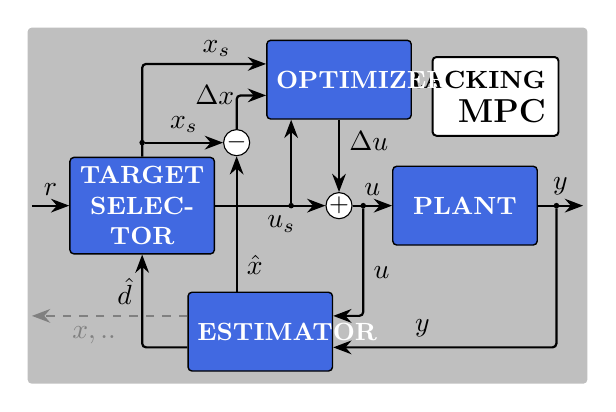
\begin{tikzpicture}[auto,
		framed, rounded corners=0.5mm,inner frame xsep = 0.4mm,outer frame sep = 0mm,
		background rectangle/.style= {fill=lightgray},
		% background grid/.style={thin, draw=gray,step=1mm}, show background grid
		% background grid/.style={draw=black,step=5mm}, show background grid
	]

	% \draw[step=1mm, style=help lines] (-32mm,-32mm) grid (34mm,34mm);
	% \node [rectangle](header)[
	% 	font=\small\bfseries\color{black},
	% 	draw=black,
	% 	line width = 0.25mm,
	% 	anchor= north west,
	% 	fill=white,
	% 	text width=8mm,
	% 	inner sep = 0mm,
	% 	rounded corners = 0.5mm,
	% 	minimum height=8mm
	% ] at (-32.5mm,20mm) {};

	\node [rectangle](title)[
		% font=\small\bfseries\color{black},
		draw=black,
		line width = 0.25mm,
		anchor=north east,
		fill=white,
		text width=16mm,
		inner sep = 0mm,
		rounded corners = 0.5mm,
		minimum height=10mm
	] at (32mm,19mm) {};
	\node (tracking)[font=\small\bfseries\color{black},
		anchor=east,] at (31.5mm,16mm) {TRACKING};
	\node (mpc)[font=\large\bfseries\color{black},
		anchor=east,] at (31.5mm,12mm) {MPC};

	\node [coordinate] (input) at (-35mm,0mm){};
	\node [coordinate] (output) at (35mm,0mm) {};
	\node [block] (t) at (-21mm,0mm){TARGET SELECTOR};
	% \node [block={black}{black}] (t) at (-21mm,0mm){TARGET SELECTOR};
	\node [sum] (x_sum) at (-9mm, 8mm) {};
	\node [dot] (x_s) at (-21mm,8mm){};
	\node at (x_sum.center){\small $\mathbf-$};
	\node [block] (o) at (4mm,16mm) {OPTIMIZER};
	\node [coordinate](o1)[above = 2mm of o.west]{};
	\node [coordinate](o2)[below = 2mm of o.west]{};
	\node [block] (e) at (-6mm,-16mm) {ESTIMATOR};
	\node [coordinate](e1)[above = 2mm of e.east]{};
	\node [coordinate](e2)[below = 2mm of e.east]{};
	\node [coordinate](e_out_1)[above = 2mm of e.west]{};
	\node [coordinate](e_out_2)[below = 2mm of e.west]{};
	\node [sum] (u_sum) at (4mm, 0mm){};
	\node at (u_sum.center){\small $\mathbf+$};
	\node [dot] (u_s) [left = 4mm of u_sum]{};
	\node [dot] (u_to_e) [right = 1mm of u_sum]{};
	\node [block] (p) at (20mm,0mm){PLANT};
	\node [dot] (y_to_e) [right = 2mm of p.east]{};

	% Arrows
	\draw [-Stealth,thick] (input) -- node {$r$} (t);

	\draw [-Stealth,thick] (t) -- node[below,pos=.6] {$u_s$} (u_sum);
	\draw [-Stealth,thick] (u_sum) -- node {$u$} (p);
	\draw [-Stealth,thick] (u_to_e) |- node[right , pos=0.3] {$u$} (e1);

	\draw [-Stealth,thick] (e.north-|x_sum.south) -- node[pos=0.2,right]  {$\hat{x}$} (x_sum);
	\draw [-Stealth,thick] (x_sum) |- node[left=-1mm]  {$\Delta x$}  (o2);
	\draw [-Stealth,thick] (x_s) -- node {$x_s$} (x_sum);
	\draw [-Stealth,thick] (t) |- node[above=.8mm, pos=.8,inner sep = 0mm] {$x_s$} (o1);

	\draw [-Stealth,thick] (o.south-|u_sum.north) -- node[pos=0.3] {$\Delta u$}  (u_sum);
	\draw [Stealth-,thick] (o.south-|u_s.north) -- node {} (u_s);

	\draw [-Stealth,thick] (p) -- node {$y$}(output);
	\draw [-Stealth,thick] (y_to_e) |- node[above,pos=.8]{$y$} (e2);
	\draw [-Stealth,thick] (e_out_2) -| node[left, pos=0.8 ] {$\hat{d}$} (t);
	\draw [-Stealth,thick,color=gray,dashed] (e_out_1) --node[pos=0.6] {\color{gray}$x,..$}  (e_out_1-|input);

\end{tikzpicture}


Tracking MPC Diagramm V2.1.tight

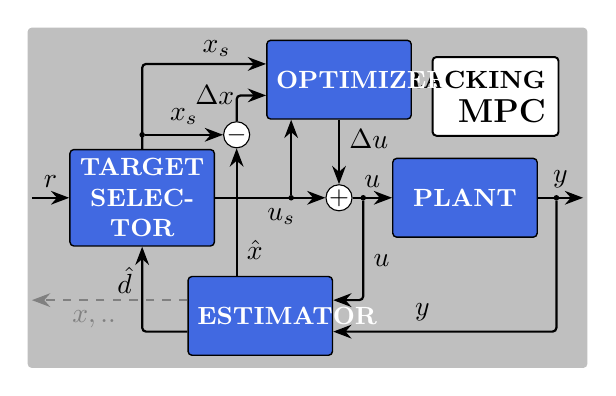
\begin{tikzpicture}[auto,
		framed, rounded corners=0.5mm,inner frame xsep = 0.4mm,outer frame sep = 0mm,
		background rectangle/.style= {fill=lightgray},
		% background grid/.style={thin, draw=gray,step=1mm}, show background grid
		% background grid/.style={draw=black,step=5mm}, show background grid
	]

	\node [rectangle](title)[
		% font=\small\bfseries\color{black},
		draw=black,
		line width = 0.25mm,
		anchor=north east,
		fill=white,
		text width=16mm,
		inner sep = 0mm,
		rounded corners = 0.5mm,
		minimum height=10mm
	] at (32mm,18mm) {};
	\node (tracking)[font=\small\bfseries\color{black},
		anchor=east,] at (31.5mm,15mm) {TRACKING};
	\node (mpc)[font=\large\bfseries\color{black},
		anchor=east,] at (31.5mm,11mm) {MPC};

	\node [coordinate] (input) at (-35mm,0mm){};
	\node [coordinate] (output) at (35mm,0mm) {};
	\node [block] (t) at (-21mm,0mm){TARGET SELECTOR};
	% \node [block={black}{black}] (t) at (-21mm,0mm){TARGET SELECTOR};
	\node [sum] (x_sum) at (-9mm, 8mm) {};
	\node [dot] (x_s) at (-21mm,8mm){};
	\node at (x_sum.center){\small $\mathbf-$};
	\node [block] (o) at (4mm,15mm) {OPTIMIZER};
	\node [coordinate](o1)[above = 2mm of o.west]{};
	\node [coordinate](o2)[below = 2mm of o.west]{};
	\node [block] (e) at (-6mm,-15mm) {ESTIMATOR};
	\node [coordinate](e1)[above = 2mm of e.east]{};
	\node [coordinate](e2)[below = 2mm of e.east]{};
	\node [coordinate](e_out_1)[above = 2mm of e.west]{};
	\node [coordinate](e_out_2)[below = 2mm of e.west]{};
	\node [sum] (u_sum) at (4mm, 0mm){};
	\node at (u_sum.center){\small $\mathbf+$};
	\node [dot] (u_s) [left = 4mm of u_sum]{};
	\node [dot] (u_to_e) [right = 1mm of u_sum]{};
	\node [block] (p) at (20mm,0mm){PLANT};
	\node [dot] (y_to_e) [right = 2mm of p.east]{};

	% Arrows
	\draw [-Stealth,thick] (input) -- node {$r$} (t);

	\draw [-Stealth,thick] (t) -- node[below,pos=.6] {$u_s$} (u_sum);
	\draw [-Stealth,thick] (u_sum) -- node {$u$} (p);
	\draw [-Stealth,thick] (u_to_e) |- node[right , pos=0.3] {$u$} (e1);

	\draw [-Stealth,thick] (e.north-|x_sum.south) -- node[pos=0.2,right]  {$\hat{x}$} (x_sum);
	\draw [-Stealth,thick] (x_sum) |- node[left=-1mm]  {$\Delta x$}  (o2);
	\draw [-Stealth,thick] (x_s) -- node {$x_s$} (x_sum);
	\draw [-Stealth,thick] (t) |- node[above=.8mm, pos=.8,inner sep = 0mm] {$x_s$} (o1);

	\draw [-Stealth,thick] (o.south-|u_sum.north) -- node[pos=0.3] {$\Delta u$}  (u_sum);
	\draw [Stealth-,thick] (o.south-|u_s.north) -- node {} (u_s);

	\draw [-Stealth,thick] (p) -- node {$y$}(output);
	\draw [-Stealth,thick] (y_to_e) |- node[above,pos=.8]{$y$} (e2);
	\draw [-Stealth,thick] (e_out_2) -| node[left, pos=0.8 ] {$\hat{d}$} (t);
	\draw [-Stealth,thick,color=gray,dashed] (e_out_1) --node[pos=0.6] {\color{gray}$x,..$}  (e_out_1-|input);

\end{tikzpicture}
